\documentclass[a4paper,11pt]{article}\usepackage[]{graphicx}\usepackage[]{color}
%% maxwidth is the original width if it is less than linewidth
%% otherwise use linewidth (to make sure the graphics do not exceed the margin)
\makeatletter
\def\maxwidth{ %
  \ifdim\Gin@nat@width>\linewidth
    \linewidth
  \else
    \Gin@nat@width
  \fi
}
\makeatother

\definecolor{fgcolor}{rgb}{0.345, 0.345, 0.345}
\newcommand{\hlnum}[1]{\textcolor[rgb]{0.686,0.059,0.569}{#1}}%
\newcommand{\hlstr}[1]{\textcolor[rgb]{0.192,0.494,0.8}{#1}}%
\newcommand{\hlcom}[1]{\textcolor[rgb]{0.678,0.584,0.686}{\textit{#1}}}%
\newcommand{\hlopt}[1]{\textcolor[rgb]{0,0,0}{#1}}%
\newcommand{\hlstd}[1]{\textcolor[rgb]{0.345,0.345,0.345}{#1}}%
\newcommand{\hlkwa}[1]{\textcolor[rgb]{0.161,0.373,0.58}{\textbf{#1}}}%
\newcommand{\hlkwb}[1]{\textcolor[rgb]{0.69,0.353,0.396}{#1}}%
\newcommand{\hlkwc}[1]{\textcolor[rgb]{0.333,0.667,0.333}{#1}}%
\newcommand{\hlkwd}[1]{\textcolor[rgb]{0.737,0.353,0.396}{\textbf{#1}}}%
\let\hlipl\hlkwb

\usepackage{framed}
\makeatletter
\newenvironment{kframe}{%
 \def\at@end@of@kframe{}%
 \ifinner\ifhmode%
  \def\at@end@of@kframe{\end{minipage}}%
  \begin{minipage}{\columnwidth}%
 \fi\fi%
 \def\FrameCommand##1{\hskip\@totalleftmargin \hskip-\fboxsep
 \colorbox{shadecolor}{##1}\hskip-\fboxsep
     % There is no \\@totalrightmargin, so:
     \hskip-\linewidth \hskip-\@totalleftmargin \hskip\columnwidth}%
 \MakeFramed {\advance\hsize-\width
   \@totalleftmargin\z@ \linewidth\hsize
   \@setminipage}}%
 {\par\unskip\endMakeFramed%
 \at@end@of@kframe}
\makeatother

\definecolor{shadecolor}{rgb}{.97, .97, .97}
\definecolor{messagecolor}{rgb}{0, 0, 0}
\definecolor{warningcolor}{rgb}{1, 0, 1}
\definecolor{errorcolor}{rgb}{1, 0, 0}
\newenvironment{knitrout}{}{} % an empty environment to be redefined in TeX

\usepackage{alltt}

\usepackage[left=2.5cm,right=2.5cm,top=3cm,bottom=3cm,pdftex]{geometry}
\usepackage{amssymb, amsmath, url, natbib, float, subcaption, listings,mathtools}
\usepackage[utf8]{inputenc}
\usepackage[T1]{fontenc}
\usepackage[pdftex]{graphicx}

\DeclareGraphicsExtensions{.png, .pdf, .jpg}
\usepackage[pdftex, colorlinks, linkcolor=blue, urlcolor=blue, citecolor=blue, pagecolor=blue, breaklinks=true]{hyperref}
\IfFileExists{upquote.sty}{\usepackage{upquote}}{}
\begin{document}

\pagestyle{empty}
\title{Comparison}
\begin{center}
\Large\textbf{CRAN packages comparison} \\[11pt]
\normalsize
\end{center}

\section{DiffusionRgqd}
Uses the cumulant truncation procedure developed by Varughese (2013), whereby the transition density can be approximated over arbitrarily large transition horizons for a suitably general class of non-linear diffusion models.

Generalized quadratic diffusions (GQD) are the specific class of SDEs with quadratic drift and diffusion terms:

\begin{align*}
d X_t & = \mu(X_t, t)dt + \sigma(X_t, t)dW_t, \: \text{where} \\
\mu(X_t, t) & = G_0(t) + G_1(t) X_t + G_2(t) X_t^2, \: \text{and} \\
\sigma (X_t, t) & = Q_0(t) + Q_1(t) X_t + Q_2(t) X_t^2
\end{align*}

For purposes of inference the drift and diffusion terms - and consequently the transitional density - are assumed to be dependent on a vector of parameters, $\theta$. For example, an Ornstein-Uhlenbeck model with SDE:

\begin{equation}
d X_t = \theta_1 (\theta_2 - X_t) + \sqrt{\theta_3^2} dW_t
\end{equation}

\begin{knitrout}
\definecolor{shadecolor}{rgb}{0.969, 0.969, 0.969}\color{fgcolor}\begin{kframe}
\begin{alltt}
\hlstd{G0}\hlkwb{=}\hlkwa{function}\hlstd{(}\hlkwc{t}\hlstd{)\{theta[}\hlnum{1}\hlstd{]}\hlopt{*}\hlstd{theta[}\hlnum{2}\hlstd{]\}}
\hlstd{G1}\hlkwb{=}\hlkwa{function}\hlstd{(}\hlkwc{t}\hlstd{)\{}\hlopt{-}\hlstd{theta[}\hlnum{1}\hlstd{]\}}
\hlstd{Q0}\hlkwb{=}\hlkwa{function}\hlstd{(}\hlkwc{t}\hlstd{)\{theta[}\hlnum{3}\hlstd{]}\hlopt{*}\hlstd{theta[}\hlnum{3}\hlstd{]\}}
\end{alltt}
\end{kframe}
\end{knitrout}

\subsection{Constant drift, diffusion SDE}
For a constant drift, diffusion SDE, with given initial condition $X_s$:
\begin{equation}
dX_t = \mu dt + \sigma dW_t
\end{equation}
The distribution at time $t$ of the process $X_t$ is $\mathcal{N}(X_t, X_s + \mu(t-s), \sigma^2(t-s))$

\begin{knitrout}
\definecolor{shadecolor}{rgb}{0.969, 0.969, 0.969}\color{fgcolor}\begin{kframe}
\begin{alltt}
\hlkwd{library}\hlstd{(}\hlstr{'DiffusionRgqd'}\hlstd{)}

\hlcom{# Remove any existing coefficients}
\hlkwd{GQD.remove}\hlstd{()}

\hlstd{Xs} \hlkwb{<-} \hlnum{0}                 \hlcom{# Initial state}
\hlstd{Xt} \hlkwb{<-} \hlkwd{seq}\hlstd{(}\hlopt{-}\hlnum{3}\hlopt{/}\hlnum{2}\hlstd{,}\hlnum{3}\hlopt{/}\hlnum{2}\hlstd{,}\hlnum{1}\hlopt{/}\hlnum{50}\hlstd{)}\hlcom{# Possible future states}
\hlstd{s}  \hlkwb{<-} \hlnum{0}                 \hlcom{# Starting time}
\hlstd{t}  \hlkwb{<-} \hlnum{1}                 \hlcom{# Final time}
\hlstd{mu}    \hlkwb{<-} \hlnum{0.5}            \hlcom{# Drift parameter}
\hlstd{sigma} \hlkwb{<-} \hlnum{0.25}           \hlcom{# Diffusion coefficient}

\hlcom{# Define the model coefficients}
\hlstd{G0} \hlkwb{<-} \hlkwa{function}\hlstd{(}\hlkwc{t}\hlstd{)\{mu\}}
\hlstd{Q0} \hlkwb{<-} \hlkwa{function}\hlstd{(}\hlkwc{t}\hlstd{)\{sigma}\hlopt{^}\hlnum{2}\hlstd{\}}

\hlcom{# Calculate the transitional density}
\hlstd{BM} \hlkwb{<-} \hlkwd{GQD.density}\hlstd{(Xs,Xt,s,t)}

\hlcom{# Plot the transitional density}
\hlkwd{plot}\hlstd{(}\hlkwd{dnorm}\hlstd{(Xt, Xs}\hlopt{+}\hlstd{mu}\hlopt{*}\hlstd{(t}\hlopt{-}\hlstd{s), sigma}\hlopt{*}\hlkwd{sqrt}\hlstd{(t}\hlopt{-}\hlstd{s))}\hlopt{~}\hlstd{Xt,} \hlkwc{main} \hlstd{=} \hlstr{'Transition density'}\hlstd{,} \hlkwc{type} \hlstd{=} \hlstr{'l'}\hlstd{)}
\hlkwd{lines}\hlstd{(BM}\hlopt{$}\hlstd{density[,}\hlnum{100}\hlstd{]}\hlopt{~}\hlstd{BM}\hlopt{$}\hlstd{Xt,} \hlkwc{col} \hlstd{=} \hlstr{'blue'}\hlstd{,} \hlkwc{lty} \hlstd{=} \hlstr{'dashed'}\hlstd{,} \hlkwc{lwd} \hlstd{=} \hlnum{2}\hlstd{)}
\end{alltt}
\end{kframe}
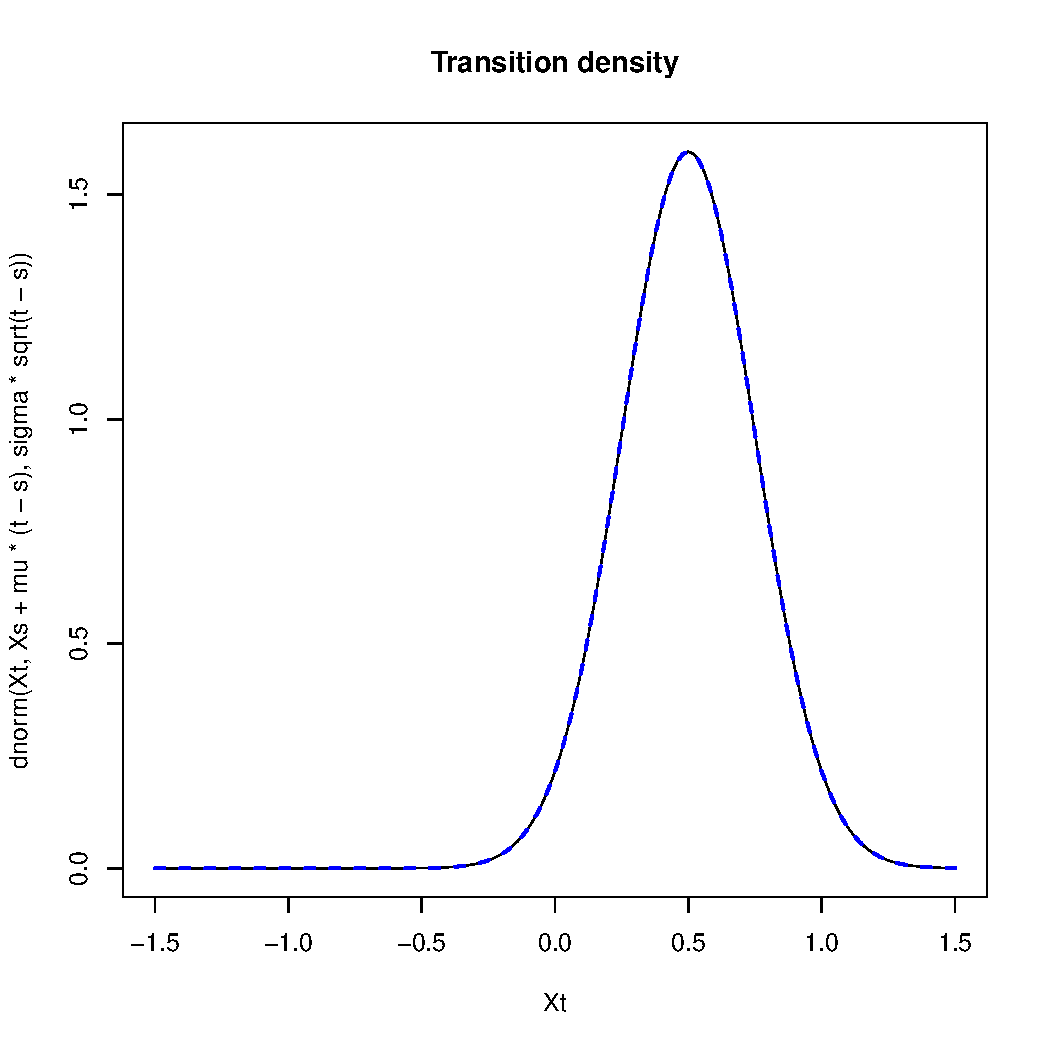
\includegraphics[width=4in,height=4in]{figure/GQD-brownian-1} 

\end{knitrout}

\subsection{CIR process}
Another example using the CIR process SDE:
\begin{equation}
dX_t = \theta_1 (\theta_2 - X_t)dt + \theta_3 \sqrt{X_t} dW_t
\end{equation}

\begin{knitrout}
\definecolor{shadecolor}{rgb}{0.969, 0.969, 0.969}\color{fgcolor}\begin{kframe}
\begin{alltt}
\hlkwd{GQD.remove}\hlstd{()}
\hlstd{a} \hlkwb{=} \hlnum{0.5}\hlstd{; b} \hlkwb{=} \hlnum{5}\hlstd{; sigma} \hlkwb{=} \hlnum{0.35}\hlstd{;} \hlcom{# Parameter values}

\hlstd{G0} \hlkwb{<-} \hlkwa{function}\hlstd{(}\hlkwc{t}\hlstd{)\{a}\hlopt{*}\hlstd{b\}}
\hlstd{G1} \hlkwb{<-} \hlkwa{function}\hlstd{(}\hlkwc{t}\hlstd{)\{}\hlopt{-}\hlstd{a\}}
\hlstd{Q1} \hlkwb{<-} \hlkwa{function}\hlstd{(}\hlkwc{t}\hlstd{)\{sigma}\hlopt{^}\hlnum{2}\hlstd{\}}

\hlstd{states}     \hlkwb{<-}  \hlkwd{seq}\hlstd{(}\hlnum{1}\hlstd{,} \hlnum{9}\hlstd{,} \hlnum{1}\hlopt{/}\hlnum{10}\hlstd{)}\hlcom{# State values}
\hlstd{initial}    \hlkwb{<-}  \hlnum{6}              \hlcom{# Starting value of the process}
\hlstd{Tmax}       \hlkwb{<-}  \hlnum{5}              \hlcom{# Time horizon}
\hlstd{Tstart}     \hlkwb{<-}  \hlnum{1}              \hlcom{# Time starts at 1}
\hlstd{increment}  \hlkwb{<-}  \hlnum{1}\hlopt{/}\hlnum{100}          \hlcom{# Incremental time steps}

\hlcom{# Generate the transitional density}
\hlstd{M} \hlkwb{<-} \hlkwd{GQD.density}\hlstd{(}\hlkwc{Xs} \hlstd{= initial,} \hlkwc{Xt} \hlstd{= states,} \hlkwc{s} \hlstd{= Tstart,} \hlkwc{t} \hlstd{= Tmax,} \hlkwc{delt} \hlstd{= increment)}

\hlkwd{persp}\hlstd{(}\hlkwc{x} \hlstd{= M}\hlopt{$}\hlstd{Xt,} \hlkwc{y} \hlstd{= M}\hlopt{$}\hlstd{time,} \hlkwc{z} \hlstd{= M}\hlopt{$}\hlstd{density,} \hlkwc{col} \hlstd{=} \hlstr{'white'}\hlstd{,} \hlkwc{xlab} \hlstd{=} \hlstr{'State (X_t)'}\hlstd{,}\hlkwc{ylab}
 \hlstd{=} \hlstr{'Time (t)'}\hlstd{,} \hlkwc{zlab} \hlstd{=} \hlstr{'Density f(X_t|X_s)'}\hlstd{,} \hlkwc{border} \hlstd{=} \hlnum{NA}\hlstd{,} \hlkwc{shade} \hlstd{=} \hlnum{0.5}\hlstd{,} \hlkwc{theta} \hlstd{=} \hlnum{145}\hlstd{)}
\end{alltt}
\end{kframe}
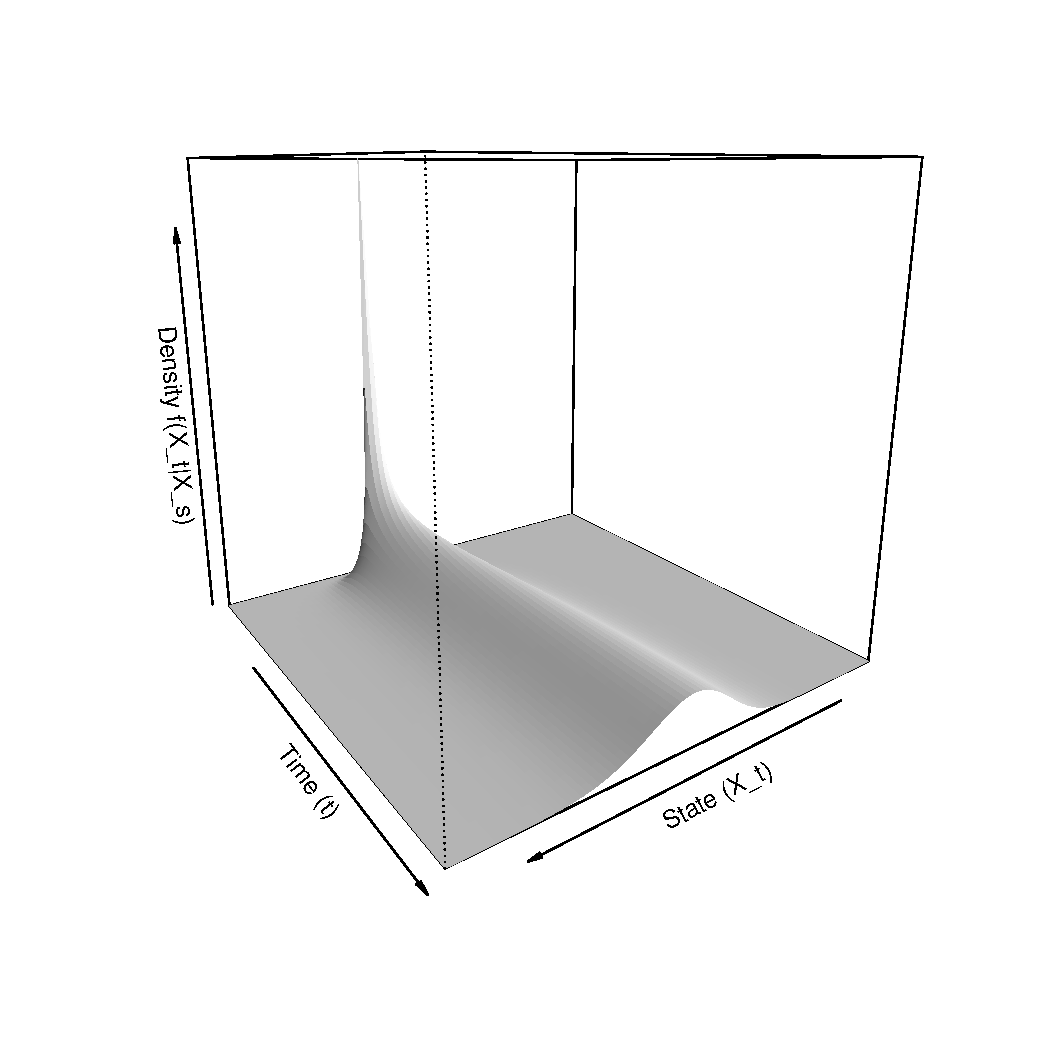
\includegraphics[width=4in,height=4in]{figure/GQD-CIR-1} 

\end{knitrout}

The GQD.density() returns (density, Xt, time, cumulants, moments, mesh). 

%The progression of mean and variance follows:
%<<GQD-meanvar, out.width='4in', out.height='4in'>>=
%plot(M$cumulants[1,]~M$time, main = 'Mean trajectory', type = 'l')
%plot(M$cumulants[2,]~M$time, main = 'Variance trajectory', type  = 'l')
%@

\subsection{Time dependent CIR process}
Consider the time-inhomogeneous CIR process for a more complicated example

\begin{equation}
dX_t = 2(10 + \sin(2 \pi (t - 0.5)) - X_t) dt + sqrt{0.25 (1 + 0.75 \sin(4 \pi t))X_t} dW_t
\end{equation}

\begin{knitrout}
\definecolor{shadecolor}{rgb}{0.969, 0.969, 0.969}\color{fgcolor}\begin{kframe}
\begin{alltt}
\hlkwd{library}\hlstd{(DiffusionRgqd)}
\hlkwd{GQD.remove}\hlstd{()}
\hlstd{G0} \hlkwb{<-} \hlkwa{function}\hlstd{(}\hlkwc{t}\hlstd{)\{}\hlnum{2}\hlopt{*}\hlstd{(}\hlnum{10}\hlopt{+}\hlkwd{sin}\hlstd{(}\hlnum{2}\hlopt{*}\hlstd{pi}\hlopt{*}\hlstd{(t}\hlopt{-}\hlnum{0.5}\hlstd{)))\}}
\hlstd{G1} \hlkwb{<-} \hlkwa{function}\hlstd{(}\hlkwc{t}\hlstd{)\{}\hlopt{-}\hlnum{2}\hlstd{\}}
\hlstd{Q1} \hlkwb{<-} \hlkwa{function}\hlstd{(}\hlkwc{t}\hlstd{)\{}\hlnum{0.25}\hlopt{*}\hlstd{(}\hlnum{1}\hlopt{+}\hlnum{0.75}\hlopt{*}\hlstd{(}\hlkwd{sin}\hlstd{(}\hlnum{4}\hlopt{*}\hlstd{pi}\hlopt{*}\hlstd{t)))\}}

\hlstd{states}    \hlkwb{<-} \hlkwd{seq}\hlstd{(}\hlnum{5}\hlstd{,} \hlnum{15}\hlstd{,} \hlnum{1}\hlopt{/}\hlnum{10}\hlstd{)}
\hlstd{initial}   \hlkwb{<-} \hlnum{8}
\hlstd{Tmax}      \hlkwb{<-} \hlnum{5}
\hlstd{Tstart}    \hlkwb{<-} \hlnum{1}
\hlstd{increment} \hlkwb{<-} \hlnum{1}\hlopt{/}\hlnum{100}

\hlstd{M} \hlkwb{<-} \hlkwd{GQD.density}\hlstd{(}\hlkwc{Xs} \hlstd{= initial,} \hlkwc{Xt} \hlstd{= states,} \hlkwc{s} \hlstd{= Tstart,} \hlkwc{t} \hlstd{= Tmax,} \hlkwc{delt} \hlstd{= increment)}
\hlkwd{persp}\hlstd{(}\hlkwc{x} \hlstd{= M}\hlopt{$}\hlstd{Xt,} \hlkwc{y} \hlstd{= M}\hlopt{$}\hlstd{time,} \hlkwc{z} \hlstd{= M}\hlopt{$}\hlstd{density,} \hlkwc{col} \hlstd{=} \hlstr{'white'}\hlstd{,} \hlkwc{xlab} \hlstd{=} \hlstr{'State (X_t)'}\hlstd{,} \hlkwc{ylab} \hlstd{=} \hlstr{'Time (t)'}\hlstd{,} \hlkwc{zlab} \hlstd{=} \hlstr{'Density f(X_t|X_s)'}\hlstd{,} \hlkwc{border} \hlstd{=} \hlnum{NA}\hlstd{,} \hlkwc{shade} \hlstd{=} \hlnum{0.5}\hlstd{,} \hlkwc{theta} \hlstd{=} \hlnum{145}\hlstd{)}
\end{alltt}
\end{kframe}
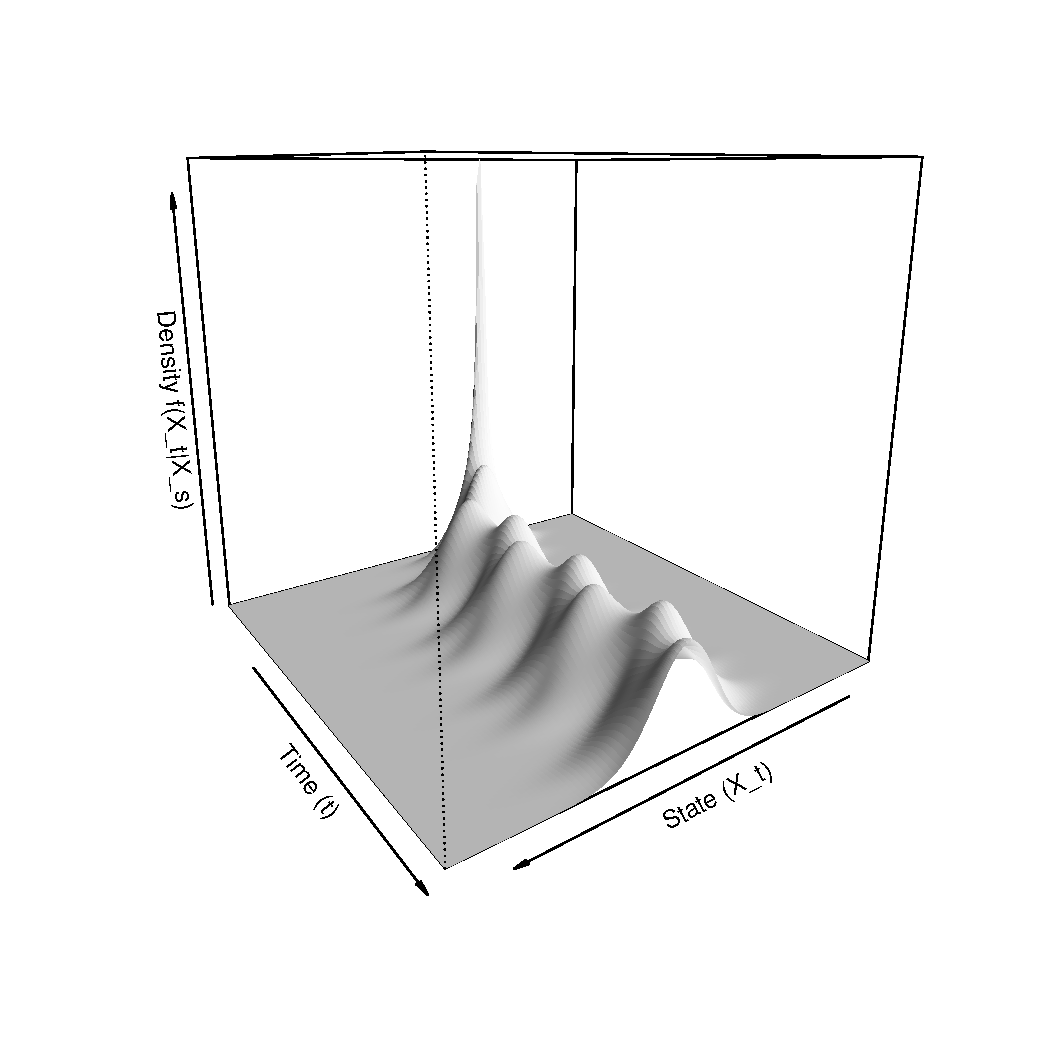
\includegraphics[width=4in,height=4in]{figure/GQD-tCIR-1} 

\end{knitrout}

\subsection{Coupled SDEs - Prey predator model}
A model that is often used to illustrate non-linear dynamics in the analysis of ODEs is that of the Lotka-Volterra model. The equations are often used to describe the dynamics of two interacting populations wherein the population growth rate of the populations are mutually influenced by the current level of the opposing population. As such the model has been used to explain oscillatory behaviour in predator-prey relationships {Hoppensteadt2006} where xtxt denotes the prey population and ytyt the predator population at time $t$. Continuing with the predator-prey metaphor, perhaps one deficiency of the model, one might argue, is the absence of random input and subsequent effects on population levels. Indeed, under the ODE formulation the predicted population behaviour (given fixed parameters) are completely deterministic. Another deficiency might be the absence of growth inhibiting factors such as disease or over-grazing. For these purposes we may define an example of a stochastic counterpart to the Lotka-Volterra equations as:

\begin{align*}
dX_t & = (aX_t - bX_t Y_t) dt + f \sqrt{X_t} dW^1_t \\
dY_t & = (-cY_t + dX_t Y_t - eY^2_t)dt + g \sqrt{Y_t} dW^2_t
\end{align*}

\begin{knitrout}
\definecolor{shadecolor}{rgb}{0.969, 0.969, 0.969}\color{fgcolor}\begin{kframe}
\begin{alltt}
\hlkwd{library}\hlstd{(DiffusionRgqd)}
\hlcom{# Remove any existing coefficients:}
\hlkwd{GQD.remove}\hlstd{()}
\end{alltt}
\begin{verbatim}
## [1] "Removed :  G0 G1 Q1"
\end{verbatim}
\begin{alltt}
\hlcom{# Define the X dimesnion coefficients:}
\hlstd{a10} \hlkwb{<-} \hlkwa{function}\hlstd{(}\hlkwc{t}\hlstd{)\{}\hlnum{1.5}\hlstd{\}}
\hlstd{a11} \hlkwb{<-} \hlkwa{function}\hlstd{(}\hlkwc{t}\hlstd{)\{}\hlopt{-}\hlnum{0.4}\hlstd{\}}
\hlstd{c10} \hlkwb{<-} \hlkwa{function}\hlstd{(}\hlkwc{t}\hlstd{)\{}\hlnum{0.05}\hlstd{\}}
\hlcom{# Define the Y dimension coefficients:}
\hlstd{b01} \hlkwb{<-} \hlkwa{function}\hlstd{(}\hlkwc{t}\hlstd{)\{}\hlopt{-}\hlnum{1.5}\hlstd{\}}
\hlstd{b11} \hlkwb{<-} \hlkwa{function}\hlstd{(}\hlkwc{t}\hlstd{)\{}\hlnum{0.4}\hlstd{\}}
\hlstd{b02} \hlkwb{<-} \hlkwa{function}\hlstd{(}\hlkwc{t}\hlstd{)\{}\hlopt{-}\hlnum{0.2}\hlstd{\}}
\hlstd{f01} \hlkwb{<-} \hlkwa{function}\hlstd{(}\hlkwc{t}\hlstd{)\{}\hlnum{0.1}\hlstd{\}}
\hlcom{# Approximate the transition density}
\hlstd{res} \hlkwb{<-} \hlkwd{BiGQD.density}\hlstd{(}\hlkwc{Xs} \hlstd{=} \hlnum{5}\hlstd{,} \hlkwc{Ys} \hlstd{=} \hlnum{5}\hlstd{,} \hlkwc{Xt} \hlstd{=} \hlkwd{seq}\hlstd{(}\hlnum{3}\hlstd{,} \hlnum{8}\hlstd{,} \hlkwc{length} \hlstd{=} \hlnum{50}\hlstd{),} \hlkwc{Yt} \hlstd{=} \hlkwd{seq}\hlstd{(}\hlnum{2}\hlstd{,} \hlnum{6}\hlstd{,} \hlkwc{length} \hlstd{=} \hlnum{50}\hlstd{),} \hlkwc{s} \hlstd{=} \hlnum{0}\hlstd{,} \hlkwc{t} \hlstd{=} \hlnum{10}\hlstd{,} \hlkwc{delt} \hlstd{=} \hlnum{1}\hlopt{/}\hlnum{100}\hlstd{)}
\end{alltt}
\begin{verbatim}
##                                                                  
##  ================================================================
##                    GENERALIZED QUADRATIC DIFFUSON                
##  ================================================================
##  _____________________ Drift Coefficients _______________________
##  a10 : 1.5                                                       
##  a11 : -0.4                                                      
##  ...   ...   ...   ...   ...   ...   ...   ...   ...   ...   ... 
##  b01 : -1.5                                                      
##  b02 : -0.2                                                      
##  b11 : 0.4                                                       
##  ___________________ Diffusion Coefficients _____________________
##  c10 : 0.05                                                      
##  ...   ...   ...   ...   ...   ...   ...   ...   ...   ...   ... 
##  ...   ...   ...   ...   ...   ...   ...   ...   ...   ...   ... 
##  ...   ...   ...   ...   ...   ...   ...   ...   ...   ...   ... 
##  f01 : 0.1                                                       
## =================================================================
\end{verbatim}
\end{kframe}
\end{knitrout}

\begin{knitrout}
\definecolor{shadecolor}{rgb}{0.969, 0.969, 0.969}\color{fgcolor}\begin{kframe}


{\ttfamily\noindent\itshape\color{messagecolor}{\#\# Loading required package: methods}}\end{kframe}
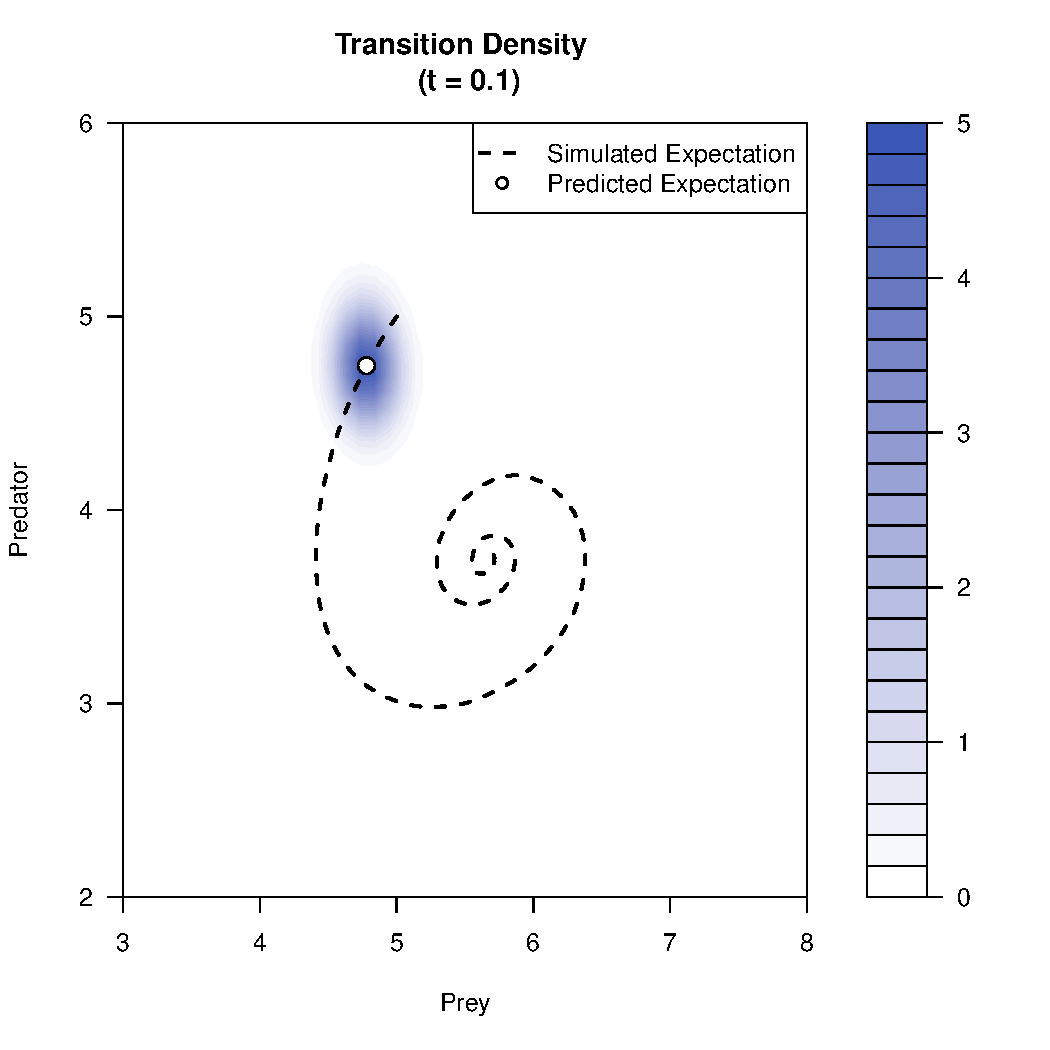
\includegraphics[width=4in,height=4in]{figure/GQD-coupledPlot-1} 

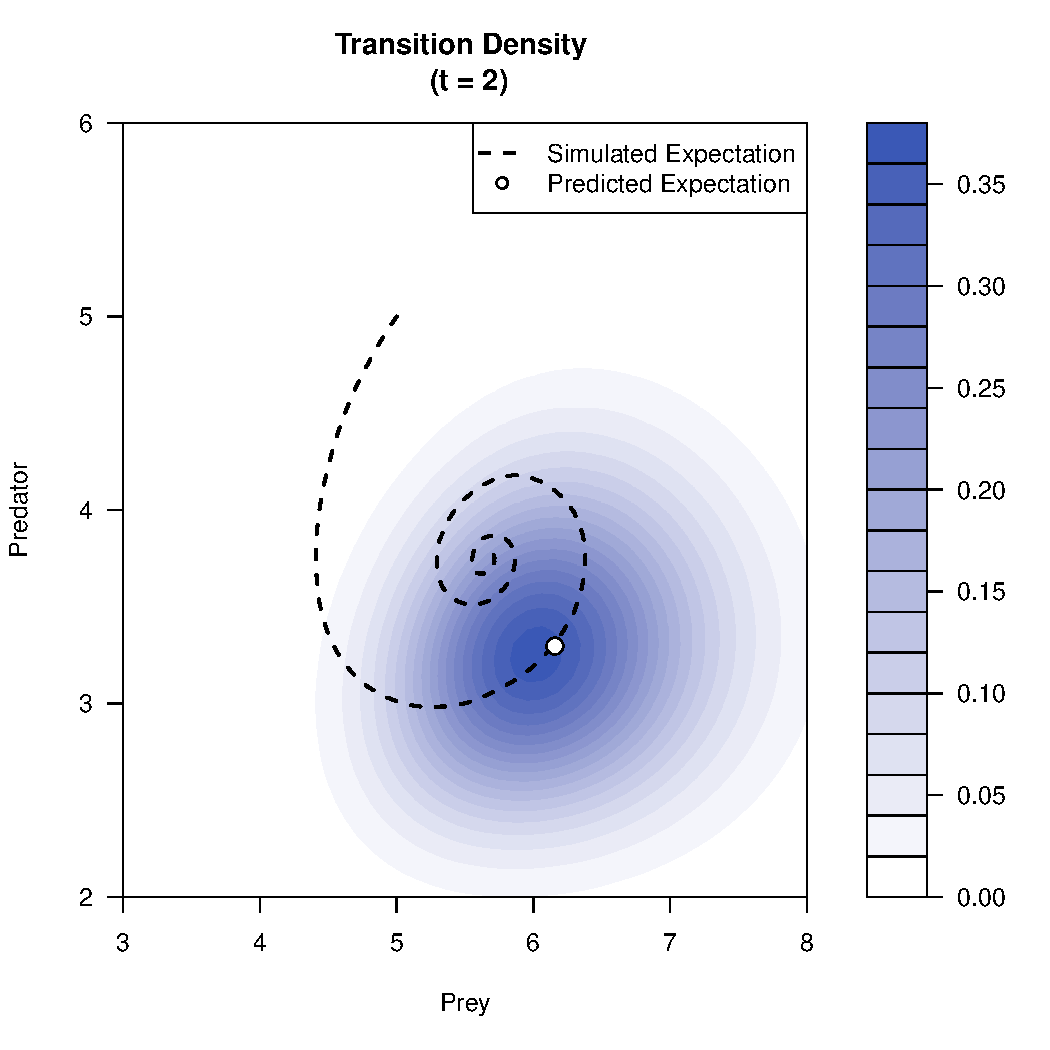
\includegraphics[width=4in,height=4in]{figure/GQD-coupledPlot-2} 

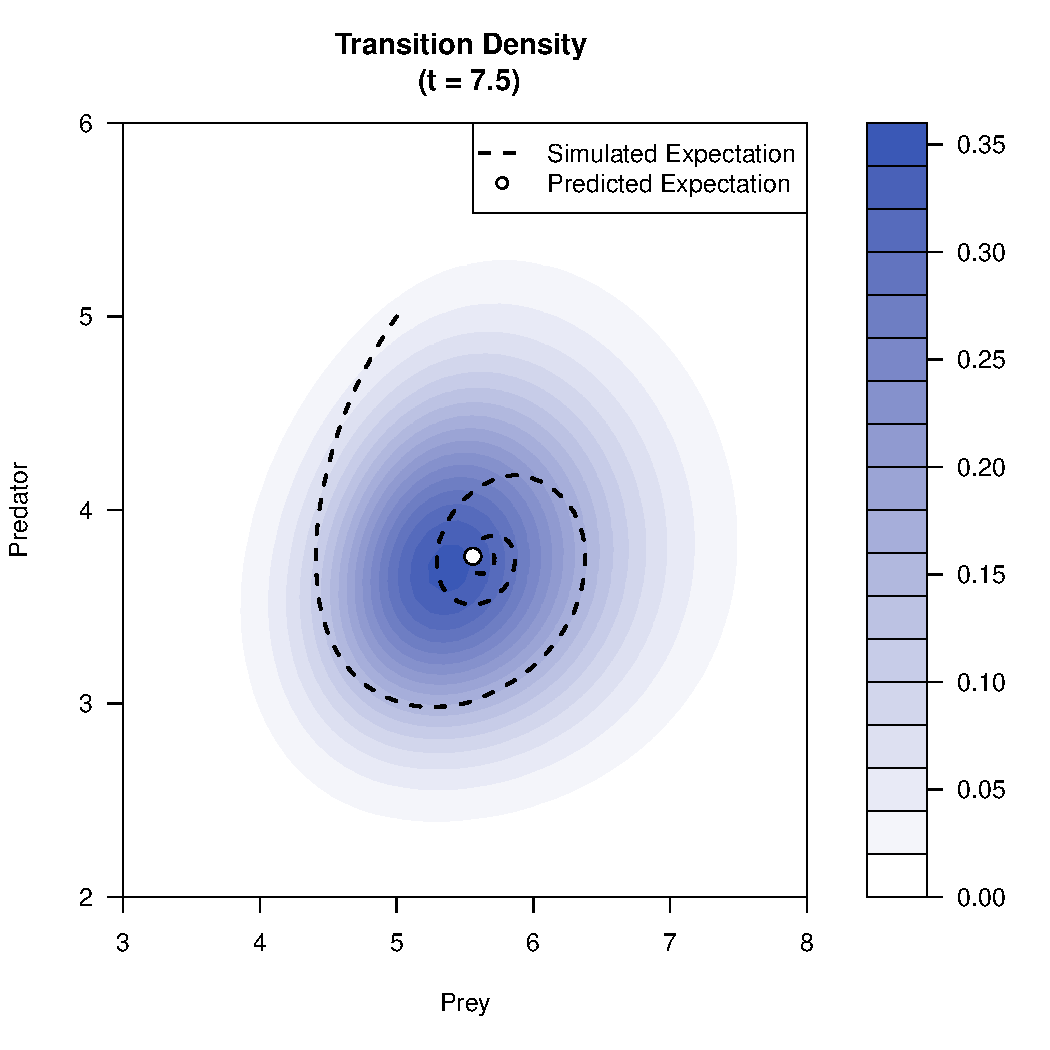
\includegraphics[width=4in,height=4in]{figure/GQD-coupledPlot-3} 

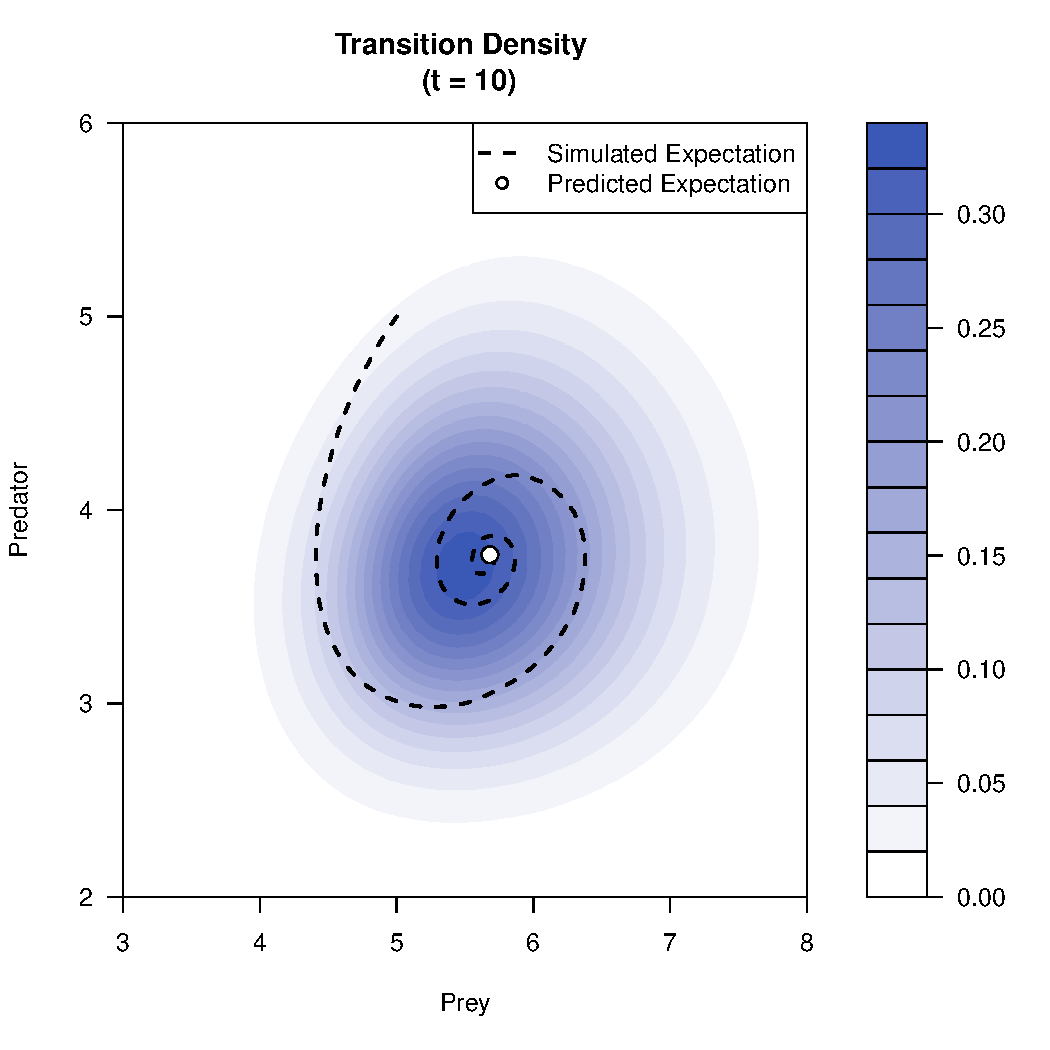
\includegraphics[width=4in,height=4in]{figure/GQD-coupledPlot-4} 

\end{knitrout}

\subsection{Inference on Diffusion Processes}
\begin{knitrout}
\definecolor{shadecolor}{rgb}{0.969, 0.969, 0.969}\color{fgcolor}\begin{kframe}
\begin{alltt}
\hlkwd{library}\hlstd{(}\hlstr{"DiffusionRgqd"}\hlstd{)}
\hlkwd{data}\hlstd{(SDEsim1)}
\hlkwd{attach}\hlstd{(SDEsim1)}
\end{alltt}


{\ttfamily\noindent\itshape\color{messagecolor}{\#\# The following object is masked \_by\_ .GlobalEnv:\\\#\# \\\#\#\ \ \ \  Xt}}

{\ttfamily\noindent\itshape\color{messagecolor}{\#\# The following object is masked from SDEsim3:\\\#\# \\\#\#\ \ \ \  time}}\begin{alltt}
\hlkwd{par}\hlstd{(}\hlkwc{mfrow}\hlstd{=}\hlkwd{c}\hlstd{(}\hlnum{1}\hlstd{,}\hlnum{1}\hlstd{))}
\hlstd{expr1}\hlkwb{=}\hlkwd{expression}\hlstd{(dX[t]}\hlopt{==}\hlnum{2}\hlopt{*}\hlstd{(}\hlnum{5}\hlopt{+}\hlnum{3}\hlopt{*}\hlkwd{sin}\hlstd{(}\hlnum{0.5}\hlopt{*}\hlstd{pi}\hlopt{*}\hlstd{t)}\hlopt{-}\hlstd{X[t])}\hlopt{*}\hlstd{dt}\hlopt{+}\hlnum{0.5}\hlopt{*}\hlkwd{sqrt}\hlstd{(X[t])}\hlopt{*}\hlstd{dW[t])}
\hlkwd{plot}\hlstd{(SDEsim1}\hlopt{$}\hlstd{Xt}\hlopt{~}\hlstd{SDEsim1}\hlopt{$}\hlstd{time,} \hlkwc{type} \hlstd{=} \hlstr{'l'}\hlstd{,} \hlkwc{col} \hlstd{=} \hlstr{'#222299'}\hlstd{,} \hlkwc{xlab} \hlstd{=} \hlstr{'Time (t)'}\hlstd{,} \hlkwc{ylab} \hlstd{=} \hlkwd{expression}\hlstd{(X[t]),} \hlkwc{main} \hlstd{= expr1)}
\end{alltt}
\end{kframe}
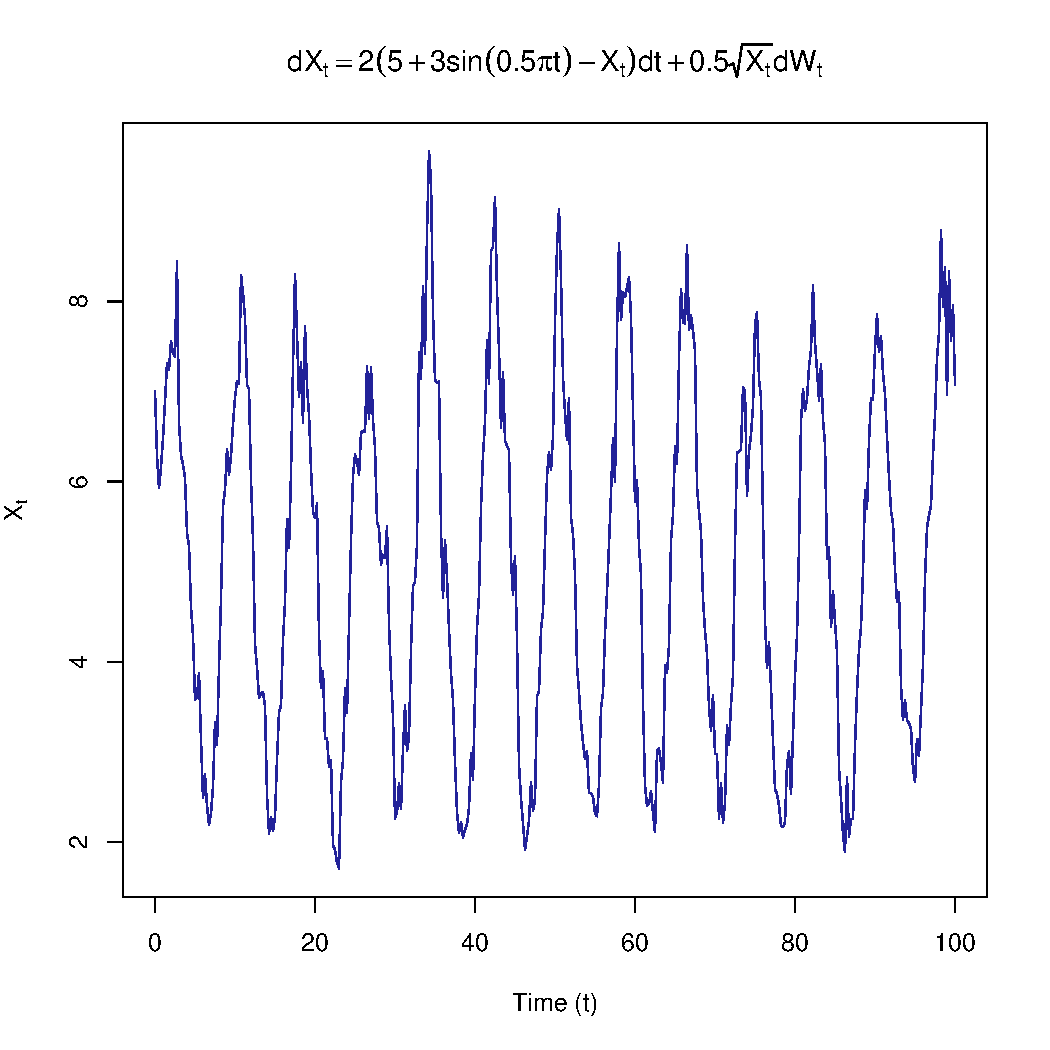
\includegraphics[width=4in]{figure/GQD-inference-1} 

\end{knitrout}

\begin{knitrout}
\definecolor{shadecolor}{rgb}{0.969, 0.969, 0.969}\color{fgcolor}\begin{kframe}
\begin{alltt}
\hlkwd{GQD.remove}\hlstd{()}

\hlstd{G0} \hlkwb{<-} \hlkwa{function}\hlstd{(}\hlkwc{t}\hlstd{)\{theta[}\hlnum{1}\hlstd{]}\hlopt{*}\hlstd{(theta[}\hlnum{2}\hlstd{]}\hlopt{+}\hlstd{theta[}\hlnum{3}\hlstd{]}\hlopt{*}\hlkwd{sin}\hlstd{(}\hlnum{0.25}\hlopt{*}\hlstd{pi}\hlopt{*}\hlstd{t))\}}
\hlstd{G1} \hlkwb{<-} \hlkwa{function}\hlstd{(}\hlkwc{t}\hlstd{)\{}\hlopt{-}\hlstd{theta[}\hlnum{1}\hlstd{]\}}
\hlstd{Q1} \hlkwb{<-} \hlkwa{function}\hlstd{(}\hlkwc{t}\hlstd{)\{theta[}\hlnum{4}\hlstd{]}\hlopt{*}\hlstd{theta[}\hlnum{4}\hlstd{]\}}

\hlstd{theta}   \hlkwb{<-} \hlkwd{c}\hlstd{(}\hlnum{1}\hlstd{,} \hlnum{10}\hlstd{,} \hlnum{1}\hlstd{,} \hlnum{1}\hlstd{)}               \hlcom{# Starting values for the chain}
\hlstd{sds}     \hlkwb{<-} \hlkwd{c}\hlstd{(}\hlnum{0.25}\hlstd{,} \hlnum{0.25}\hlstd{,} \hlnum{0.2}\hlstd{,} \hlnum{0.05}\hlstd{)}\hlopt{/}\hlnum{1.5} \hlcom{# Std devs for proposal distributions}
\hlstd{mesh}    \hlkwb{<-} \hlnum{10}                           \hlcom{# Number of mesh points}
\hlstd{updates} \hlkwb{<-} \hlnum{110000}                       \hlcom{# Perform 110000 updates}
\hlstd{burns}   \hlkwb{<-} \hlnum{10000}                        \hlcom{# Burn 10000 updates}

\hlcom{# Run the MCMC procedure for the model defined above:}
\hlstd{model_1} \hlkwb{<-} \hlkwd{GQD.mcmc}\hlstd{(SDEsim1}\hlopt{$}\hlstd{Xt, SDEsim1}\hlopt{$}\hlstd{time, mesh, theta, sds, updates, burns)}
\end{alltt}
\end{kframe}
\end{knitrout}

% TODO: Fix input

% <<GQD-RanOnRSeparately>>=
% _____________________ Drift Coefficients _______________________
% G0 : theta[1]*(theta[2]+theta[3]*sin(0.25*pi*t))                
% G1 : -theta[1]                                                  
% G2                                                              
% ___________________ Diffusion Coefficients _____________________
% Q0                                                              
% Q1 : theta[4]*theta[4]                                          
% Q2                                                              
% _____________________ Prior Distributions ______________________
                                                             
% d(theta):None.                                                  
% @

% TODO: Add the inference plot

The estimates are given by

\begin{knitrout}
\definecolor{shadecolor}{rgb}{0.969, 0.969, 0.969}\color{fgcolor}\begin{kframe}
\begin{alltt}
\hlkwd{GQD.estimates}\hlstd{(model_1,} \hlkwc{thin} \hlstd{=} \hlnum{100}\hlstd{,} \hlkwc{burns} \hlstd{=} \hlnum{10000}\hlstd{,} \hlkwc{corrmat} \hlstd{=} \hlnum{TRUE}\hlstd{)}
\end{alltt}
\end{kframe}
\end{knitrout}

% TODO: Fix the results
% <<GQD-estimatesResult>>=
%          Estimate lower_CI upper_CI
% theta[1]    2.026    1.820    2.256
% theta[2]    5.016    4.922    5.106
% theta[3]    2.915    2.787    3.050
% theta[4]    0.501    0.472    0.534

% $corrmat
%          theta[1] theta[2] theta[3] theta[4]
% theta[1]     1.00    -0.19    -0.36     0.38
% theta[2]    -0.19     1.00     0.35    -0.03
% theta[3]    -0.36     0.35     1.00    -0.13
% theta[4]     0.38    -0.03    -0.13     1.00
% @

% TODO: Add the trace plot

\section{pomp: statistical inference for partially-observed Markov processes}
POMP focuses on partially observed Markov process models or hidden Markov models. They consist of an observed process $Y_n$ from the system and an unobserved process $X_n$ controlled by a stochastic process. The stochastic process model is determined by the density $f_{X_n | X_{n-1}}$. Following the R convention, in the pomp package the simulation of $f_{X_n|X_{n-1}}$ (the process model) is referred to as the $\textit{rprocess}$ whereas the evaluation of $f_{X_n|X_{n-1}}$ is referred as the $\textit{dprocess}$. Similarly, for the measurement process, $f_{Y_n|X_n}$, the simulation component is $\textit{rmeasure}$, while the evaluation component is called $\textit{dmeasure}$.


\section{Robfilter}

\section{Sim.DiffProc Package - PMLE}
Pseudo-maximum likelihood estimators for one-dimensional SDEs. The four schemes implemented are: $\textbf{Euler}$, $\textbf{Ozaki}$, $\textbf{Shoji-Ozaki}$, $\textbf{Kessler}$ method. These methods don't approximate the transition density directly but the path of the process $X_t$ in such a way that the discretized version of the process has a usable likelihood. \\

Consider the general form of the SDE:
\begin{equation}
dX_t = f(X_t, t, \theta)dt + g(X_t, t, \theta)dWt
\end{equation}
An assumption is made that the infinitesimal coefficients don't depend on $t$, so the equation can be approximated as
\begin{equation}
dX_t = f(X_t, \theta) dt + g(X_t, \theta)dW_t
\end{equation}
where $X_t$ is considered a time-homogeneous process. Using the above assumption, the transition density can be approximated as $p(\Delta t, x, y) = p(t_{i-1}, x, y, t_i)$. Given initial conditions $X_0$ and $\theta_0$, the log likelihood function is 
\begin{align*}
l_n (\theta) = \sum_{i=1}^{n} log p_{\theta} (\Delta t, X_{i-1}, X_i) + log p_{\theta} (X_0)
\end{align*}
The PMLE (pseudo maximum likelihood estimator) $\tilde{\theta}_n = \arg \max h_n(\theta | X_1, \cdots, X_n)$ is estimated from a density $h$ that doesn't belong to the family of the true conditional density but is compatible with the moments with $p$ (??). This method applied to high frequency data, i.e. $\Delta t \to 0, n\Delta t \to \infty$.


\section{HPloglik}

\section{abctools}

\section{sde (Stefano 2015)} 

\section{yuima (Stefano 2014)}
Simulation and inference for multidimensional SDEs

\section{PSM package (Stig and Soren 2013)}
Estimation of linear and non-linear mixed-effects models using SDEs. Also uses filtering to find smoothed estimates for the model states. It allow any multivariate non-linear time-variant model and had the ability to handle missing observations. Kalman filtering is used for linear models. \\

A mixed-effects model is used wherein the variation is split into intra-individual variation and inter-individual variation using a 2 stage model. The first stage model is a state space model consisting of a continuous state equation and defined by the dynamics of the system and a set of discrete measurement equations which defines the relation between the obtained observations and the system observations.

\begin{align*}
dx_t & = (A(\phi_i) x_t + B(\phi_i) u_t)dt + \sigma_{\omega}(\phi_i) d \omega_t \\
y_{ij} & = C(\phi_i) x_{ij} + D(\phi_i) u_{ij} + e_{ij}
\end{align*}

For a general non-linear model, the system is specified as
\begin{align*}
dx_t & = f(\phi_i, x_t, u_t, t)dt + \sigma(\phi_i, u_t, t) d \omega_t \\
y_{ij} & = g(\phi_i, u_{ij}, x_{ij}, t_{ij}) + e_{ij}
\end{align*}
where $t$ is a continuous variable and in multivariable case, the state and measurement variables can be denoted as a vector at time $t_{ij}$. The noise is assumed to follow Gaussian noise $e_{ij} \in \mathcal{N}(0, S(\phi_i, u_t, t))$, where $S$ denotes the covariance matrix. The model parameters are denoted by $\phi_i$. \\

For the model evaluation, it requires computations of the Jacobian matrix with first order partial derivatives, $\frac{\partial f}{\partial x_t}$ and $\frac{\partial g}{\partial x_t}$. \\

The second stage model describes the variation of the model parameters $\phi_i$ between individuals,

\begin{align*}
\phi_i = h(\theta, \eta_i, Z_i)
\end{align*}
where $\eta_i$ is the multivariate random effect parameter for the $i^{th}$ parameter and is assumed Gaussian, i.e., $\eta_i \in \mathcal{N}(0, \Omega)$

\subsection{Parameter Estimation}
Maximum likelihood estimator is used for parameter estimation. The full set of model parameters to be estimated are the matrices $\Sigma, \sigma_{\omega}, \Omega, \theta$. The likelihood function is approximated by a second-order Taylor expansion around the value of $\hat{\eta_i}$ that maximizes it.
\begin{align*}
- \log L(\Theta) \approx \sum_{i=1}^N \frac{1}{2} \log \Bigg|\frac{-\Delta l_i}{2 \pi}\Bigg| - l_i
\end{align*}

This likelihood function is evaluated using the Kalman filter which gives an exact solution for linear models. For non-linear models, the Extended Kalman filter is used which is only an approximation. There are 4 types of state and state covariance estimates available using the EKF, each of which differs in the way data is used:

\begin{enumerate}
\item Simulation estimate: $\hat{x}_{i(j|0)}, \hat{P}_{i(j|0)}$ \\
estimate of the state evolution for repeated experiments without updating based on measurements, yields a confidence band for the state evolution
\item Prediction estimate: $\hat{x}_{i(j|j-1)}, \hat{P}_{i(j|j-1)}$ \\
prediction required to give the conditional density for the next observation at time $t_{ij}$ given the observations upto $t_{i(j|j-1)}$
\item Filtering estimate : $\hat{x}_{i(j|j)}, \hat{P}_{i(j|j)}$ \\
best estimate at time $t_{ij}$ given the observations upto time $t_{ij}$ 
\item Smoothing estimate: $\hat{x}_{i(j|N)}, \hat{P}_{i(j|N)}$ \\
optimal estimate at time $t_{ij}$ utilizing all observations both prior and after the time $t_{ij}$
\end{enumerate}

There are 2 key objects in the packages, data object and model object. The data object contains sample times, observations and inputs while the model object contains everything else related to the model.

\begin{knitrout}
\definecolor{shadecolor}{rgb}{0.969, 0.969, 0.969}\color{fgcolor}\begin{kframe}
\begin{alltt}
\hlkwd{library}\hlstd{(}\hlstr{'PSM'}\hlstd{)}
\hlkwd{PSM.template}\hlstd{(}\hlkwc{Linear}\hlstd{=}\hlnum{TRUE}\hlstd{,}\hlkwc{dimX}\hlstd{=}\hlnum{3}\hlstd{,}\hlkwc{dimY}\hlstd{=}\hlnum{1}\hlstd{,}\hlkwc{dimU}\hlstd{=}\hlnum{0}\hlstd{,}\hlkwc{dimEta}\hlstd{=}\hlnum{3}\hlstd{)}
\end{alltt}
\begin{verbatim}
## 
## 
## MyModel <- vector(mode="list")
## MyModel$Matrices=function(phi) {
##   list(
##        matA=matrix(c(  ), nrow=3, ncol=3),
##        matC=matrix(c(  ), nrow=1, ncol=3)
##        )
## }
## MyModel$h = function(eta,theta,covar) {
##   phi <- theta
##   phi
## }
## MyModel$S = function(phi) {
##   matrix(c(  ), nrow=1, ncol=1)
## }
## MyModel$SIG = function(phi) {
##   matrix(c(  ), nrow=3, ncol=3)
## }
## MyModel$X0 = function(Time,phi,U) {
##   matrix(c(  ), nrow=3, ncol=1)
## }
## MyModel$ModelPar = function(THETA) {
##   list(theta=list(  ),
##        OMEGA=matrix(c(  ), nrow=3, ncol=3)
##        )
## }
\end{verbatim}
\end{kframe}
\end{knitrout}

The data object is a list with the following components:
\begin{enumerate}
\item $Y$ - the matrix with observations, columns hold multivariate observations at a time point, missing observations entered as NA
\item $Time$ - sample times, same number of columns in $Y$
\end{enumerate}

\begin{knitrout}
\definecolor{shadecolor}{rgb}{0.969, 0.969, 0.969}\color{fgcolor}\begin{kframe}
\begin{alltt}
\hlstd{MyData} \hlkwb{<-} \hlkwd{list}\hlstd{()}
\hlstd{MyData[[}\hlnum{1}\hlstd{]]} \hlkwb{<-} \hlkwd{list}\hlstd{(}\hlkwc{Time}\hlstd{=}\hlnum{1}\hlopt{:}\hlnum{4}\hlstd{,}\hlkwc{Y}\hlstd{=}\hlkwd{matrix}\hlstd{(}\hlkwd{c}\hlstd{(}\hlnum{2.1}\hlstd{,}\hlnum{3.2}\hlstd{,}\hlnum{3.4}\hlstd{,}\hlnum{3.7}\hlstd{),}\hlkwc{nrow}\hlstd{=}\hlnum{1}\hlstd{),}\hlkwc{covar}\hlstd{=}\hlkwd{c}\hlstd{(}\hlkwc{BMI}\hlstd{=}\hlnum{20.1}\hlstd{))}
\hlstd{MyData[[}\hlnum{2}\hlstd{]]} \hlkwb{<-} \hlkwd{list}\hlstd{(}\hlkwc{Time}\hlstd{=}\hlnum{3}\hlopt{:}\hlnum{7}\hlstd{,}\hlkwc{Y}\hlstd{=}\hlkwd{matrix}\hlstd{(}\hlkwd{c}\hlstd{(}\hlnum{1.9}\hlstd{,}\hlnum{2.1}\hlstd{,}\hlnum{2.0}\hlstd{,}\hlnum{2.9}\hlstd{,}\hlnum{3.5}\hlstd{),}\hlkwc{nrow}\hlstd{=}\hlnum{1}\hlstd{),}\hlkwc{covar}\hlstd{=}\hlkwd{c}\hlstd{(}\hlkwc{BMI}\hlstd{=}\hlnum{23.4}\hlstd{))}
\end{alltt}
\end{kframe}
\end{knitrout}

Main functions for parameter estimation include:
\begin{enumerate}
\item PSM.estimate(Model, Data, THETA, deltaTime)
\item PSM.estimate(Model, Data, Par, CI)
\item PSM.smooth(Model, Data, THETA, subsample)
\item PSM.plot(Data, Smooth, indiv, type)
\item PSM.template(Linear,dimX,dimY,dimU,dimEta,file)
\end{enumerate}

\subsection{Linear Coupled SDE (Dosing in two-compartment model)}
\begin{align*}
dA_1 & = \Bigg( - \frac{CL}{V_1^i}A_1 - \frac{CL_d}{V_1^i}A_1 + \frac{CL_d}{V_2}A_2\Bigg) dt + \sigma_1 d\omega \\
dA_2 & = \Bigg( \frac{CL_d}{V_1^i}A_1 - \frac{CL_d}{V_2}A_2\Bigg)dt - \sigma_1 d \omega \\
Y & = \frac{A_1}{V_1^i} + e
\end{align*}

\begin{knitrout}
\definecolor{shadecolor}{rgb}{0.969, 0.969, 0.969}\color{fgcolor}\begin{kframe}
\begin{alltt}
\hlstd{Model.SimDose} \hlkwb{=} \hlkwd{list}\hlstd{()}

\hlstd{Model.SimDose}\hlopt{$}\hlstd{Matrices} \hlkwb{=} \hlkwa{function}\hlstd{(}\hlkwc{phi}\hlstd{)}
\hlstd{\{}
        \hlstd{V1i} \hlkwb{<-} \hlstd{phi}\hlopt{$}\hlstd{V1i; V2}\hlkwb{=}\hlstd{phi}\hlopt{$}\hlstd{V2; CL} \hlkwb{=} \hlstd{phi}\hlopt{$}\hlstd{CL; CLd} \hlkwb{=} \hlstd{phi}\hlopt{$}\hlstd{CLd;}
        \hlstd{matA} \hlkwb{<-} \hlkwd{matrix}\hlstd{(}\hlkwd{c}\hlstd{(}\hlopt{-}\hlstd{(CL}\hlopt{+}\hlstd{CLd)}\hlopt{/}\hlstd{V1i , CLd}\hlopt{/}\hlstd{V2 , CLd}\hlopt{/}\hlstd{V1i ,} \hlopt{-}\hlstd{CLd}\hlopt{/}\hlstd{V2 ) ,}\hlkwc{nrow}\hlstd{=}\hlnum{2}\hlstd{,}\hlkwc{byrow}\hlstd{=T)}
        \hlstd{matC} \hlkwb{<-} \hlkwd{matrix}\hlstd{(}\hlkwd{c}\hlstd{(}\hlnum{1}\hlopt{/}\hlstd{V1i,}\hlnum{0}\hlstd{),}\hlkwc{nrow}\hlstd{=}\hlnum{1}\hlstd{)}
        \hlkwd{list}\hlstd{(}\hlkwc{matA}\hlstd{=matA,}\hlkwc{matC}\hlstd{=matC)}
\hlstd{\}}

\hlstd{Model.SimDose}\hlopt{$}\hlstd{X0} \hlkwb{=} \hlkwa{function}\hlstd{(}\hlkwc{Time}\hlstd{=Na,}\hlkwc{phi}\hlstd{,}\hlkwc{U}\hlstd{=Na) \{} \hlkwd{matrix}\hlstd{(}\hlnum{0}\hlstd{,}\hlkwc{nrow}\hlstd{=}\hlnum{2}\hlstd{) \}}

\hlstd{Model.SimDose}\hlopt{$}\hlstd{SIG} \hlkwb{=} \hlkwa{function}\hlstd{(}\hlkwc{phi}\hlstd{)}
\hlstd{\{}
        \hlstd{sig1} \hlkwb{<-} \hlstd{phi[[}\hlstr{"sig1"}\hlstd{]]}
        \hlkwd{matrix}\hlstd{(}\hlkwd{c}\hlstd{( sig1,}\hlnum{0}\hlstd{,}\hlopt{-}\hlstd{sig1,}\hlnum{0}\hlstd{),} \hlkwc{nrow}\hlstd{=}\hlnum{2}\hlstd{,} \hlkwc{byrow}\hlstd{=T)}
\hlstd{\}}

\hlstd{Model.SimDose}\hlopt{$}\hlstd{S} \hlkwb{=} \hlkwa{function}\hlstd{(}\hlkwc{phi}\hlstd{) \{} \hlkwd{matrix}\hlstd{(phi[[}\hlstr{"S"}\hlstd{]]) \}}

\hlstd{Model.SimDose}\hlopt{$}\hlstd{h} \hlkwb{=} \hlkwa{function}\hlstd{(}\hlkwc{eta}\hlstd{,}\hlkwc{theta}\hlstd{,}\hlkwc{covar}\hlstd{)}
\hlstd{\{}
        \hlstd{phi} \hlkwb{<-} \hlstd{theta}
        \hlstd{phi}\hlopt{$}\hlstd{V1i} \hlkwb{<-} \hlstd{theta}\hlopt{$}\hlstd{V1}\hlopt{*}\hlkwd{exp}\hlstd{(eta[}\hlnum{1}\hlstd{])}
        \hlstd{phi}
\hlstd{\}}

\hlstd{Model.SimDose}\hlopt{$}\hlstd{ModelPar} \hlkwb{=} \hlkwa{function}\hlstd{(}\hlkwc{THETA}\hlstd{)}
\hlstd{\{}
        \hlstd{V2} \hlkwb{<-} \hlnum{10}
        \hlstd{CLd} \hlkwb{<-} \hlnum{0.1}
        \hlkwd{list}\hlstd{(}\hlkwc{theta}\hlstd{=}\hlkwd{list}\hlstd{(}\hlkwc{V1} \hlstd{= THETA[}\hlstr{'V1'}\hlstd{],}\hlkwc{V2}\hlstd{=V2,}\hlkwc{CLd}\hlstd{=CLd,}\hlkwc{CL}\hlstd{=THETA[}\hlstr{'CL'}\hlstd{],} \hlkwc{sig1}\hlstd{=THETA[}\hlstr{'sig1'}\hlstd{],} \hlkwc{S}\hlstd{=THETA[}\hlstr{'S'}\hlstd{]),}
        \hlkwc{OMEGA}\hlstd{=}\hlkwd{matrix}\hlstd{(THETA[}\hlstr{'OMEGA1'}\hlstd{]) )}
\hlstd{\}}

\hlstd{SimDose.THETA} \hlkwb{<-} \hlkwd{c}\hlstd{(}\hlkwc{CL}\hlstd{=}\hlnum{0.05}\hlstd{,}\hlkwc{V1} \hlstd{=} \hlnum{5}\hlstd{,} \hlkwc{sig1} \hlstd{=} \hlnum{10} \hlstd{,} \hlkwc{S} \hlstd{=} \hlnum{20} \hlstd{,} \hlkwc{OMEGA1} \hlstd{=} \hlnum{.2}\hlstd{)}

\hlstd{N} \hlkwb{=} \hlnum{5}
\hlstd{SimDose.Data} \hlkwb{<-} \hlkwd{vector}\hlstd{(}\hlkwc{mode}\hlstd{=}\hlstr{"list"}\hlstd{,}\hlkwc{length}\hlstd{=N)}
\hlkwa{for} \hlstd{(i} \hlkwa{in} \hlnum{1}\hlopt{:}\hlstd{N)}
\hlstd{\{}
        \hlstd{SimDose.Data[[i]]}\hlopt{$}\hlstd{Time} \hlkwb{<-} \hlkwd{seq}\hlstd{(}\hlkwc{from}\hlstd{=}\hlnum{10}\hlstd{,}\hlkwc{by}\hlstd{=}\hlnum{10}\hlstd{,}\hlkwc{to}\hlstd{=}\hlnum{400}\hlstd{)}
        \hlstd{SimDose.Data[[i]]}\hlopt{$}\hlstd{Dose} \hlkwb{<-}\hlkwd{list}\hlstd{(}\hlkwc{Time} \hlstd{=} \hlkwd{c}\hlstd{(}\hlnum{30}\hlstd{,}\hlnum{180}\hlstd{),} \hlkwc{State} \hlstd{=} \hlkwd{c}\hlstd{(}\hlnum{1}\hlstd{,} \hlnum{1}\hlstd{),} \hlkwc{Amount} \hlstd{=} \hlkwd{c}\hlstd{(}\hlnum{1500}\hlstd{,}\hlnum{1500}\hlstd{))}
\hlstd{\}}
\end{alltt}
\end{kframe}
\end{knitrout}

The previous code is for setting up the parameters. Now the simulation and plotting can be done as follows:

\begin{knitrout}
\definecolor{shadecolor}{rgb}{0.969, 0.969, 0.969}\color{fgcolor}\begin{kframe}
\begin{alltt}
\hlstd{SimDose.Data} \hlkwb{<-} \hlkwd{PSM.simulate}\hlstd{(Model.SimDose, SimDose.Data, SimDose.THETA,} \hlkwc{deltaTime}\hlstd{=}\hlnum{.1}\hlstd{)}
\end{alltt}
\begin{verbatim}
## Simulating individual: 1, 2, 3, 4, 5, Done
\end{verbatim}
\begin{alltt}
\hlkwd{PSM.plot}\hlstd{(SimDose.Data,}\hlkwc{indiv}\hlstd{=}\hlnum{1}\hlopt{:}\hlnum{2}\hlstd{,}\hlkwc{type}\hlstd{=}\hlkwd{c}\hlstd{(}\hlstr{'Y'}\hlstd{,}\hlstr{'longX'}\hlstd{,}\hlstr{'eta'}\hlstd{))}
\end{alltt}
\end{kframe}
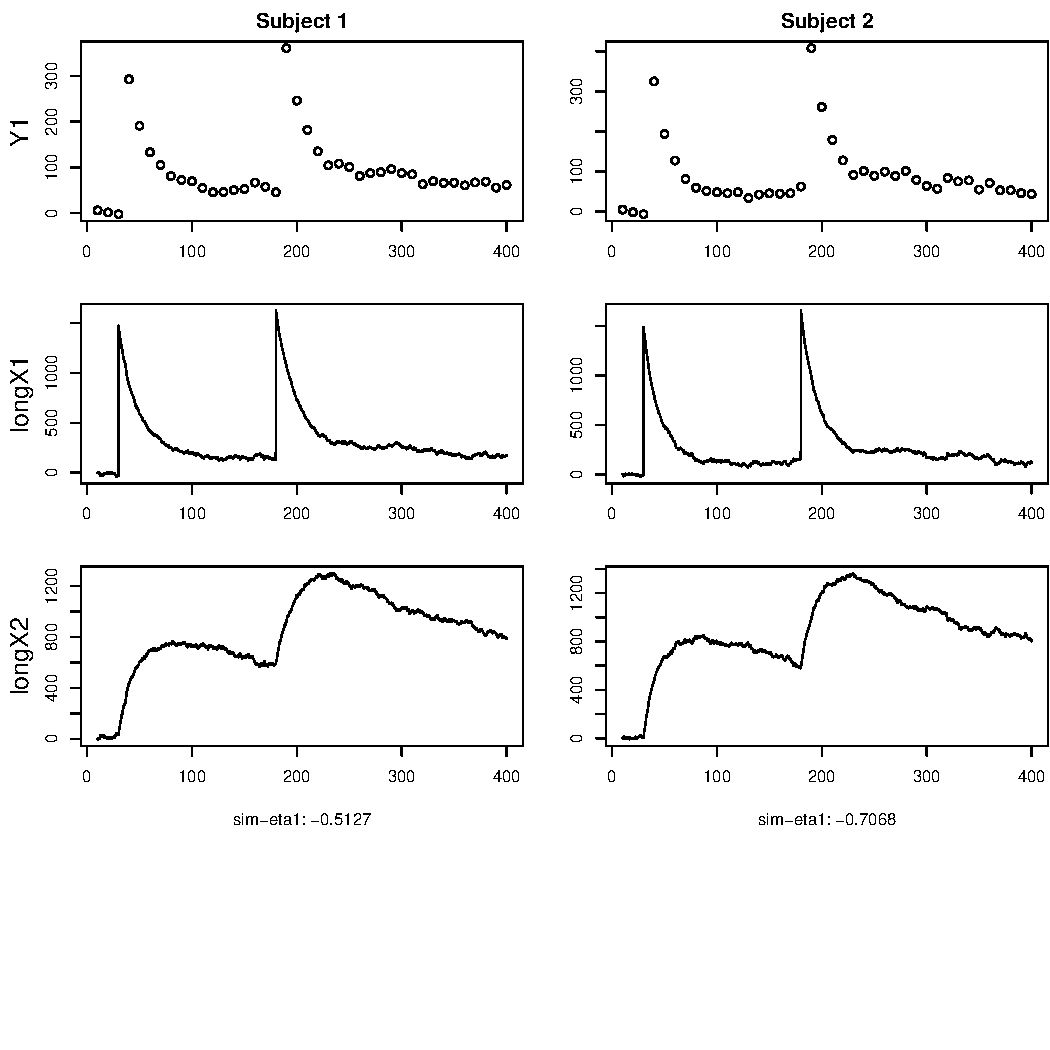
\includegraphics[width=\maxwidth]{figure/PSM_simulate-1} 

\end{knitrout}

\begin{knitrout}
\definecolor{shadecolor}{rgb}{0.969, 0.969, 0.969}\color{fgcolor}\begin{kframe}
\begin{alltt}
\hlstd{parA} \hlkwb{<-} \hlkwd{list}\hlstd{(}\hlkwc{LB}\hlstd{=SimDose.THETA}\hlopt{*}\hlnum{.5}\hlstd{,} \hlkwc{Init}\hlstd{=SimDose.THETA ,} \hlkwc{UB}\hlstd{=SimDose.THETA}\hlopt{*}\hlnum{1.5} \hlstd{)}
\hlstd{fitA} \hlkwb{<-} \hlkwd{PSM.estimate}\hlstd{(Model.SimDose,SimDose.Data,parA,}\hlkwc{CI}\hlstd{=T)}
\hlstd{fitA[}\hlnum{1}\hlopt{:}\hlnum{5}\hlstd{]}
\end{alltt}
\begin{verbatim}
## $NegLogL
## [1] 701.3212
## 
## $THETA
##          CL          V1        sig1           S      OMEGA1 
##  0.05024533  3.61376844  8.44487780 19.44636937  0.10104120 
## 
## $CI
##                    CL       V1      sig1         S     OMEGA1
## Lower CI95 0.04899241 2.601711  6.623071  7.340308 -0.1462456
## MLE        0.05024533 3.613768  8.444878 19.446369  0.1010412
## Upper CI95 0.05149825 4.625826 10.266685 31.552431  0.3483280
## 
## $SD
##               CL        V1      sig1        S    OMEGA1
## [1,] 0.000639244 0.5163558 0.9294934 6.176562 0.1261668
## 
## $COR
##                  CL           V1         sig1           S       OMEGA1
## CL      1.000000000 -0.008943151  0.052756970 -0.05303231 -0.015988479
## V1     -0.008943151  1.000000000  0.007180018  0.00391188 -0.005626545
## sig1    0.052756970  0.007180018  1.000000000 -0.68857347 -0.044245905
## S      -0.053032310  0.003911880 -0.688573474  1.00000000  0.038325727
## OMEGA1 -0.015988479 -0.005626545 -0.044245905  0.03832573  1.000000000
\end{verbatim}
\begin{alltt}
\hlstd{SimDose.THETA}
\end{alltt}
\begin{verbatim}
##     CL     V1   sig1      S OMEGA1 
##   0.05   5.00  10.00  20.00   0.20
\end{verbatim}
\end{kframe}
\end{knitrout}

Based on the estimated parameters, it is possible to obtain a smoothes estimate of the model states

\begin{knitrout}
\definecolor{shadecolor}{rgb}{0.969, 0.969, 0.969}\color{fgcolor}\begin{kframe}
\begin{alltt}
\hlstd{out} \hlkwb{<-} \hlkwd{PSM.smooth}\hlstd{(Model.SimDose, SimDose.Data, fitA}\hlopt{$}\hlstd{THETA,} \hlkwc{subsample} \hlstd{=} \hlnum{20}\hlstd{)}
\hlkwd{names}\hlstd{(out[[}\hlnum{1}\hlstd{]])}
\end{alltt}
\begin{verbatim}
##  [1] "Time"    "Xs"      "Ps"      "Ys"      "Xf"      "Pf"      "Xp"     
##  [8] "Pp"      "Yp"      "R"       "eta"     "negLogL"
\end{verbatim}
\end{kframe}
\end{knitrout}


\end{document}

